% 图 6.23 畴结构选择：(a)单畴强退磁场 (b)双畴 (c)封闭畴(磁通闭合)
\documentclass[tikz,border=5pt]{standalone}
\usetikzlibrary{arrows.meta}
\usepackage{amsmath}
\usepackage{bm}
\usepackage{fontspec}
\setmainfont{Times New Roman}
\begin{document}
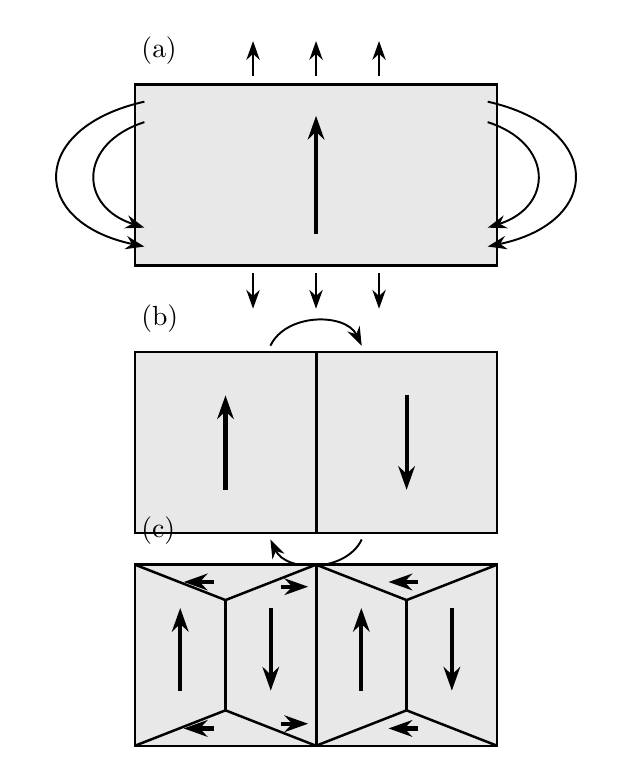
\begin{tikzpicture}[line width=0.8pt,>=Stealth,
  mag/.style={->,line width=1.5pt,>={Stealth[length=3mm,width=2.1mm]}},
  fld/.style={->,line width=0.7pt,>={Stealth[length=2.4mm,width=1.7mm]}}]
% ================= (a) single domain =================
\node[anchor=south west] at (-0.05,8.52) {(a)};
\fill[gray!18] (0,6.1) rectangle (4.6,8.4);
\draw[line width=0.9pt] (0,6.1) rectangle (4.6,8.4);
\draw[mag] (2.3,6.5) -- (2.3,8.0);
% external dipolar field: side loops (arrows pointing down)
\draw[fld] (0.12,8.18) .. controls (-1.35,7.85) and (-1.35,6.65) .. (0.12,6.34);
\draw[fld] (0.12,7.92) .. controls (-0.72,7.65) and (-0.72,6.85) .. (0.12,6.58);
\draw[fld] (4.48,8.18) .. controls (5.95,7.85) and (5.95,6.65) .. (4.48,6.34);
\draw[fld] (4.48,7.92) .. controls (5.32,7.65) and (5.32,6.85) .. (4.48,6.58);
% stray field arrows at top and bottom
\foreach \xx in {1.5,2.3,3.1} {
  \draw[fld] (\xx,8.5) -- (\xx,8.95);
  \draw[fld] (\xx,6.0) -- (\xx,5.55);
}
% ================= (b) two domains =================
\node[anchor=south west] at (-0.05,5.12) {(b)};
\fill[gray!18] (0,2.7) rectangle (4.6,5.0);
\draw[line width=0.9pt] (0,2.7) rectangle (4.6,5.0);
\draw[line width=1.1pt] (2.3,2.7) -- (2.3,5.0);
\draw[mag] (1.15,3.25) -- (1.15,4.45);
\draw[mag] (3.45,4.45) -- (3.45,3.25);
% small flux loops above and below
\draw[fld] (1.72,5.08) .. controls (1.92,5.5) and (2.68,5.5) .. (2.88,5.08);
\draw[fld] (2.88,2.62) .. controls (2.68,2.2) and (1.92,2.2) .. (1.72,2.62);
% ================= (c) closure domains =================
\node[anchor=south west] at (-0.05,2.42) {(c)};
\fill[gray!18] (0,0) rectangle (4.6,2.3);
\draw[line width=0.9pt] (0,0) rectangle (4.6,2.3);
% main domain walls
\draw[line width=1.1pt] (1.15,0.45) -- (1.15,1.85);
\draw[line width=1.1pt] (2.3,0) -- (2.3,2.3);
\draw[line width=1.1pt] (3.45,0.45) -- (3.45,1.85);
% closure-domain slant walls (top)
\draw[line width=0.9pt] (0,2.3) -- (1.15,1.85) -- (2.3,2.3) -- (3.45,1.85) -- (4.6,2.3);
% closure-domain slant walls (bottom)
\draw[line width=0.9pt] (0,0) -- (1.15,0.45) -- (2.3,0) -- (3.45,0.45) -- (4.6,0);
% main domain arrows: up down up down
\draw[mag] (0.575,0.7)  -- (0.575,1.75);
\draw[mag] (1.725,1.75) -- (1.725,0.7);
\draw[mag] (2.875,0.7)  -- (2.875,1.75);
\draw[mag] (4.025,1.75) -- (4.025,0.7);
% closure arrows: top left right left
\draw[mag] (1.0,2.08) -- (0.62,2.08);
\draw[mag] (1.85,2.02) -- (2.2,2.02);
\draw[mag] (3.6,2.08) -- (3.22,2.08);
% closure arrows: bottom left right left
\draw[mag] (1.0,0.22) -- (0.62,0.22);
\draw[mag] (1.85,0.28) -- (2.2,0.28);
\draw[mag] (3.6,0.22) -- (3.22,0.22);
\end{tikzpicture}
\end{document}
